%\VignetteIndexEntry{LEA: An R Package for Landscape and Ecological Association Studies}

\documentclass[12pt,a4paper,oneside]{article}\usepackage[]{graphicx}\usepackage[]{color}
%% maxwidth is the original width if it is less than linewidth
%% otherwise use linewidth (to make sure the graphics do not exceed the margin)
\makeatletter
\def\maxwidth{ %
  \ifdim\Gin@nat@width>\linewidth
    \linewidth
  \else
    \Gin@nat@width
  \fi
}
\makeatother

\definecolor{fgcolor}{rgb}{0.345, 0.345, 0.345}
\newcommand{\hlnum}[1]{\textcolor[rgb]{0.686,0.059,0.569}{#1}}%
\newcommand{\hlstr}[1]{\textcolor[rgb]{0.192,0.494,0.8}{#1}}%
\newcommand{\hlcom}[1]{\textcolor[rgb]{0.678,0.584,0.686}{\textit{#1}}}%
\newcommand{\hlopt}[1]{\textcolor[rgb]{0,0,0}{#1}}%
\newcommand{\hlstd}[1]{\textcolor[rgb]{0.345,0.345,0.345}{#1}}%
\newcommand{\hlkwa}[1]{\textcolor[rgb]{0.161,0.373,0.58}{\textbf{#1}}}%
\newcommand{\hlkwb}[1]{\textcolor[rgb]{0.69,0.353,0.396}{#1}}%
\newcommand{\hlkwc}[1]{\textcolor[rgb]{0.333,0.667,0.333}{#1}}%
\newcommand{\hlkwd}[1]{\textcolor[rgb]{0.737,0.353,0.396}{\textbf{#1}}}%
\let\hlipl\hlkwb

\usepackage{framed}
\makeatletter
\newenvironment{kframe}{%
 \def\at@end@of@kframe{}%
 \ifinner\ifhmode%
  \def\at@end@of@kframe{\end{minipage}}%
  \begin{minipage}{\columnwidth}%
 \fi\fi%
 \def\FrameCommand##1{\hskip\@totalleftmargin \hskip-\fboxsep
 \colorbox{shadecolor}{##1}\hskip-\fboxsep
     % There is no \\@totalrightmargin, so:
     \hskip-\linewidth \hskip-\@totalleftmargin \hskip\columnwidth}%
 \MakeFramed {\advance\hsize-\width
   \@totalleftmargin\z@ \linewidth\hsize
   \@setminipage}}%
 {\par\unskip\endMakeFramed%
 \at@end@of@kframe}
\makeatother

\definecolor{shadecolor}{rgb}{.97, .97, .97}
\definecolor{messagecolor}{rgb}{0, 0, 0}
\definecolor{warningcolor}{rgb}{1, 0, 1}
\definecolor{errorcolor}{rgb}{1, 0, 0}
\newenvironment{knitrout}{}{} % an empty environment to be redefined in TeX

\usepackage{alltt}

\usepackage{natbib}
\IfFileExists{upquote.sty}{\usepackage{upquote}}{}
\begin{document}




\title{{\tt LEA}: An {\tt R} Package for Landscape and Ecological Association Studies}
\author{Eric Frichot and Olivier Fran\c{c}ois \\ 
Universit\'e Grenoble-Alpes,\\ Centre National de la Recherche Scientifique, \\
TIMC-IMAG UMR 5525, Grenoble, 38042, France.
}
\date{}
\maketitle
\tableofcontents

\section{Overview}
{\tt LEA} \citep{Frichot_2015} is an {\tt R} package dedicated to landscape genomics and
    ecological association tests. {\tt LEA} can run analyses of
        population structure and genomewide tests for local adaptation. 
        The package includes statistical methods for estimating ancestry
        coefficients from large genotypic matrices and for evaluating the
        number of ancestral populations (snmf, pca). It performs statistical 
        tests using latent factor mixed models for identifying
        genetic polymorphisms that exhibit high correlation with
        environmental gradients (lfmm). {\tt LEA} is mainly based on optimized C programs
        that can scale with the dimension of large data sets.  


\section{Introduction} 
The goal of this tutorial is to give an overview of the main  functionalities of the {\tt R} package {\tt LEA}. It will show the main steps of analysis, including 1) analysing population structure and preparing a genotypic matrix for genomewide association studies, 2) fitting GWAS latent factor mixed models to the data and extracting candidate regions of interest.    

As some functions may take a few hours to analyse very large datasets, output files are written into text files that can be read by {\tt LEA} after each batch of runs (called a 'project'). We advise creating working directories containing genotypic data and covariables when starting {\tt LEA}. Note that two files with the same names but a different extension are assumed to contain the same data in distinct formats.

\begin{knitrout}
\definecolor{shadecolor}{rgb}{0.969, 0.969, 0.969}\color{fgcolor}\begin{kframe}
\begin{alltt}
\hlcom{# creation of a directory for LEA analyses}
\hlkwd{dir.create}\hlstd{(}\hlstr{"LEA_analyses"}\hlstd{)}
\hlcom{# set the created directory as the working directory}
\hlkwd{setwd}\hlstd{(}\hlstr{"LEA_analyses"}\hlstd{)}
\end{alltt}
\end{kframe}
\end{knitrout}

\newline
\newline
The tutorial dataset is a quite small dataset that consists of 400 SNPs genotyped for 50 diploids individuals. The last 50 SNPs are correlated with an environmental variable, and represent the targets of the LEA analysis. Similar artificial data were analyzed in the computer note introducing the R package LEA \citep{Frichot_2015}. 

\begin{knitrout}
\definecolor{shadecolor}{rgb}{0.969, 0.969, 0.969}\color{fgcolor}\begin{kframe}
\begin{alltt}
\hlkwd{library}\hlstd{(LEA)}
\hlcom{# Creation a the genotypic file: "genotypes.lfmm"}
\hlcom{# The data include 400 SNPs for 50 individuals.}
\hlkwd{data}\hlstd{(}\hlstr{"tutorial"}\hlstd{)}
\hlcom{# Write genotypes in the lfmm format}
\hlkwd{write.lfmm}\hlstd{(tutorial.R,} \hlstr{"genotypes.lfmm"}\hlstd{)}
\hlcom{# Write genotypes in the geno format}
\hlkwd{write.geno}\hlstd{(tutorial.R,} \hlstr{"genotypes.geno"}\hlstd{)}
\hlcom{# creation of an environment gradient file: gradient.env.}
\hlcom{# The .env file contains a single ecological variable}
\hlcom{# for each individual.}
\hlkwd{write.env}\hlstd{(tutorial.C,} \hlstr{"gradients.env"}\hlstd{)}
\end{alltt}
\end{kframe}
\end{knitrout}

\newline
\newline
Note that the {\tt LEA} package is to be able to handle very large population 
genetic data sets. Genomic data are processed using fast C codes wrapped into the {\tt R} code. Most {\tt LEA} functions use character strings containing paths to input files as arguments.

\subsection{Input files}
The {\tt R} package {\tt LEA} can handle several input file formats for genotypic matrices. More specifically, the package uses the {\tt lfmm} and {\tt geno} formats, and provides functions to convert from other formats such as {\tt ped}, {\tt vcf}, and {\tt ancestrymap} formats. The program VCFTOOLS can be very useful in providing one of those format ({\tt ped} is the closest to an {\tt lfmm} matrix).
\newline
\newline
The {\tt lfmm} and {\tt geno} formats can also be used for coding multiallelic marker data (eg, microsatellites). For those data, the conversion function {\tt struct2geno} converts files in the STRUCTURE format in the  {\tt geno} or {\tt lfmm} formats. {\tt LEA} can also process allele frequency data if they are encoded in the {\tt lfmm} format. In that case, the {\tt lfmm} function will use allele counts for populations in its model. 
\newline
\newline
Phenotypic traits and ecological predictors must be formatted in the {\tt env} format. This format corresponds to a matrix where each variable is represented as a column \citep{Frichot_2013}. It uses the {\tt .env} extension.
\newline
\newline
When using ecological data, we often need to decide which variables should be used among a large number of ecological indicators (eg, climatic variables), we suggest that users summarize their data using linear combinations of those indicators. Considering principal component analysis and using the first principal components as proxies for ecological gradients linked to selective forces can be useful in this context.
\newline
\newline
The {\tt LEA} package can handle missing data in population structure analyses. In association analyses, missing genotypes must be replaced by imputed values using a missing data imputation method. We encourage users to remove their missing data by using the function {\tt impute()}, which is based on population structure analysis(see next section). Note that specialized genotype imputation programs such as BEAGLE, IMPUTE2 or MENDEL-IMPUTE could provide better imputation results than {\tt LEA}. Filtering out rare variants -- retaining minor allele frequency greater than 5 percent --, and removing regions in strong LD may also result in better analyses with {\tt LEA}.


\section{Analysis of population structure and missing data imputation}

The {\tt R} package {\tt LEA} implements two classical approaches for the estimation of population genetic structure: principal component analysis (pca) and admixture analysis \citep{Patterson_2006, Pritchard_2000a} using nonnegative matrix factorization (snmf). The algorithms programmed in {\tt LEA} are improved versions of pca and admixture analysis able to process very large genotypic matrices efficiently.

\subsection{Principal Component Analysis}

The {\tt LEA} function {\tt pca} computes the scores of a pca for a genotypic matrix, and returns a scree-plot for the eigenvalues of the sample covariance matrix. Using {\tt pca}, an object of class {\tt pcaProject} is created. This object contains a path to the files storing eigenvectors, eigenvalues and projections. 

\begin{knitrout}
\definecolor{shadecolor}{rgb}{0.969, 0.969, 0.969}\color{fgcolor}\begin{kframe}
\begin{alltt}
\hlcom{# run of pca}
\hlcom{# Available options, K (the number of PCs), }
\hlcom{#                    center and scale. }
\hlcom{# Create files: genotypes.eigenvalues - eigenvalues,        }
\hlcom{#               genotypes.eigenvectors - eigenvectors,}
\hlcom{#               genotypes.sdev - standard deviations,}
\hlcom{#               genotypes.projections - projections,}
\hlcom{# Create a pcaProject object: pc.}
\hlstd{pc} \hlkwb{=} \hlkwd{pca}\hlstd{(}\hlstr{"genotypes.lfmm"}\hlstd{,} \hlkwc{scale} \hlstd{=} \hlnum{TRUE}\hlstd{)}
\end{alltt}
\end{kframe}
\end{knitrout}
\noindent
The number of "significant" components can be evaluated using graphical methods based on the screeplot (Figure 1). The knee in the screeplot indicates that there
are around $K = 4$ major components in the data ($\approx 5$ genetic clusters). 
Following  \citep{Patterson_2006}, the {\tt tracy.widom} function computes Tracy-Widom tests for each eigenvalue as follows.

\begin{knitrout}
\definecolor{shadecolor}{rgb}{0.969, 0.969, 0.969}\color{fgcolor}\begin{kframe}
\begin{alltt}
\hlcom{# Perfom Tracy-Widom tests on all eigenvalues.}
\hlcom{# create file: tuto.tracyWidom - tracy-widom test information.  }
\hlstd{tw} \hlkwb{=} \hlkwd{tracy.widom}\hlstd{(pc)}
\end{alltt}
\end{kframe}
\end{knitrout}

\begin{knitrout}
\definecolor{shadecolor}{rgb}{0.969, 0.969, 0.969}\color{fgcolor}\begin{kframe}
\begin{alltt}
\hlcom{# display p-values for the Tracy-Widom tests (first 10 pcs). }
\hlstd{tw}\hlopt{$}\hlstd{pvalues[}\hlnum{1}\hlopt{:}\hlnum{10}\hlstd{]}
\end{alltt}
\begin{verbatim}
##  [1] 8.000e-09 8.000e-09 8.000e-09 1.503e-04 3.152e-02 4.215e-01 6.565e-01
##  [8] 6.859e-01 6.738e-01 9.363e-01
\end{verbatim}
\end{kframe}
\end{knitrout}

\begin{figure}[h!]
    \centering
\begin{knitrout}
\definecolor{shadecolor}{rgb}{0.969, 0.969, 0.969}\color{fgcolor}\begin{kframe}
\begin{alltt}
\hlcom{# plot the percentage of variance explained by each component}
\hlkwd{plot}\hlstd{(tw}\hlopt{$}\hlstd{percentage)}
\end{alltt}
\end{kframe}
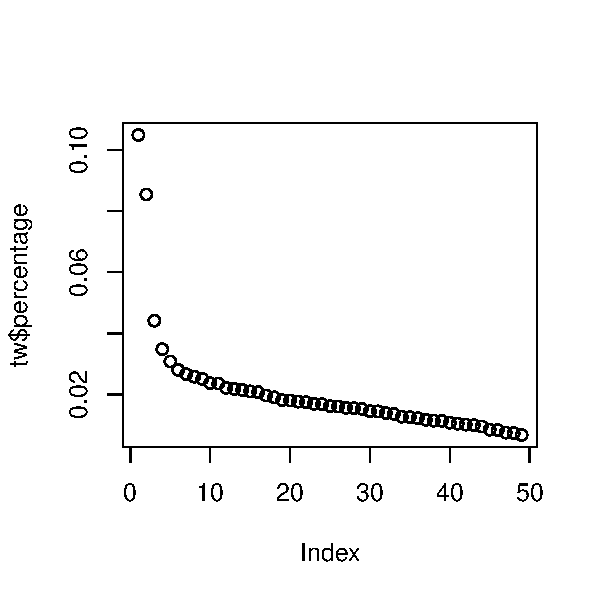
\includegraphics[width=\maxwidth]{figure/unnamed-chunk-7-1} 

\end{knitrout}
\caption{Screeplot for the percentage of variance explained by each component in PCA of the genetic data. The knee at $K = 4$ indicates that their 5 major genetic clusters in the data.}
\end{figure}


\subsection{Inference of individual admixture coefficients using {\tt snmf}}

{\tt LEA} includes the {\tt R} function {\tt snmf} that estimates individual admixture coefficients from the genotypic matrix with provides results very close to Bayesian clustering programs \citep{Pritchard_2000a, Francois_2010}. Assuming $K$ ancestral populations, the {\tt R} function {\tt snmf} provides least-squares estimates of ancestry proportions \citep{Frichot_2014}. 

\begin{knitrout}
\definecolor{shadecolor}{rgb}{0.969, 0.969, 0.969}\color{fgcolor}\begin{kframe}
\begin{alltt}
\hlcom{# main options}
\hlcom{# K = number of ancestral populations}
\hlcom{# entropy = TRUE: computes the cross-entropy criterion, }
\hlcom{# CPU = 4 the number of CPUs.}
\hlstd{project} \hlkwb{=} \hlkwa{NULL}
\hlstd{project} \hlkwb{=} \hlkwd{snmf}\hlstd{(}\hlstr{"genotypes.geno"}\hlstd{,}
               \hlkwc{K} \hlstd{=} \hlnum{1}\hlopt{:}\hlnum{10}\hlstd{,}
               \hlkwc{entropy} \hlstd{=} \hlnum{TRUE}\hlstd{,}
               \hlkwc{repetitions} \hlstd{=} \hlnum{10}\hlstd{,}
               \hlkwc{project} \hlstd{=} \hlstr{"new"}\hlstd{)}
\end{alltt}
\end{kframe}
\end{knitrout}


The {\tt snmf} function estimates an entropy criterion that evaluates the quality of fit of the statistical model to the data using a cross-validation technique (Figure 2). The entropy criterion can help choosing the number of ancestral populations that best explains the genotypic data \citep{Alexander_2011, Frichot_2014}. Here we have a clear minimum at $K = 4$, suggesting 4 genetic clusters. Often, the plot shows a less clear pattern, and choosing the "knee" is a generally good approach. The number of ancestral populations is closely linked to the number of principal components that explain variation in the genomic data. Both numbers can help determining the number of latent factors when correcting for confounding effects due to population structure in ecological association tests. 

\begin{figure}[h!]
    \centering
\begin{knitrout}
\definecolor{shadecolor}{rgb}{0.969, 0.969, 0.969}\color{fgcolor}\begin{kframe}
\begin{alltt}
\hlcom{# plot cross-entropy criterion for all runs in the snmf project}
\hlkwd{plot}\hlstd{(project,} \hlkwc{lwd} \hlstd{=} \hlnum{5}\hlstd{,} \hlkwc{col} \hlstd{=} \hlstr{"blue"}\hlstd{,} \hlkwc{pch} \hlstd{=} \hlnum{1}\hlstd{)}
\end{alltt}
\end{kframe}
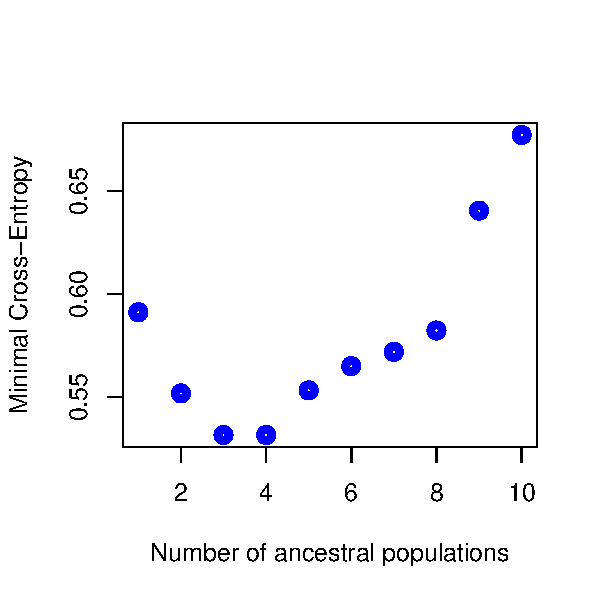
\includegraphics[width=\maxwidth]{figure/unnamed-chunk-9-1} 

\end{knitrout}
\caption{Value of the cross-entropy criterion as a function
of the number of populations in {\tt snmf}.}
\end{figure}

The next step is to display a barplot for the $Q$-matrix. Here, the {\tt Q} function is called and its output is converted into a {\tt Qmatrix} object. 
\begin{figure}[h!]
    \centering
\begin{knitrout}
\definecolor{shadecolor}{rgb}{0.969, 0.969, 0.969}\color{fgcolor}\begin{kframe}
\begin{alltt}
\hlcom{# select the best run for K = 4}
\hlstd{best} \hlkwb{=} \hlkwd{which.min}\hlstd{(}\hlkwd{cross.entropy}\hlstd{(project,} \hlkwc{K} \hlstd{=} \hlnum{4}\hlstd{))}
\hlstd{Q.matrix} \hlkwb{<-} \hlkwd{as.qmatrix}\hlstd{(}\hlkwd{Q}\hlstd{(project,} \hlkwc{K} \hlstd{=} \hlnum{4}\hlstd{,} \hlkwc{run} \hlstd{= best))}
\hlstd{my.colors} \hlkwb{<-} \hlkwd{c}\hlstd{(}\hlstr{"tomato"}\hlstd{,} \hlstr{"lightblue"}\hlstd{,}
               \hlstr{"olivedrab"}\hlstd{,} \hlstr{"gold"}\hlstd{)}
\hlkwd{barplot}\hlstd{(Q.matrix,} \hlkwc{border} \hlstd{=} \hlnum{NA}\hlstd{,} \hlkwc{space} \hlstd{=} \hlnum{0}\hlstd{,}
        \hlkwc{col} \hlstd{= my.colors,}
        \hlkwc{xlab} \hlstd{=} \hlstr{"Individuals"}\hlstd{,}
        \hlkwc{ylab} \hlstd{=} \hlstr{"Ancestry proportions"}\hlstd{,}
        \hlkwc{main} \hlstd{=} \hlstr{"Ancestry matrix"}\hlstd{)} \hlkwb{->} \hlstd{bp}
\hlkwd{axis}\hlstd{(}\hlnum{1}\hlstd{,} \hlkwc{at} \hlstd{=} \hlnum{1}\hlopt{:}\hlkwd{nrow}\hlstd{(Q.matrix),}
     \hlkwc{labels} \hlstd{= bp}\hlopt{$}\hlstd{order,} \hlkwc{las} \hlstd{=} \hlnum{3}\hlstd{,}
     \hlkwc{cex.axis} \hlstd{=} \hlnum{.7}\hlstd{)}
\end{alltt}
\end{kframe}
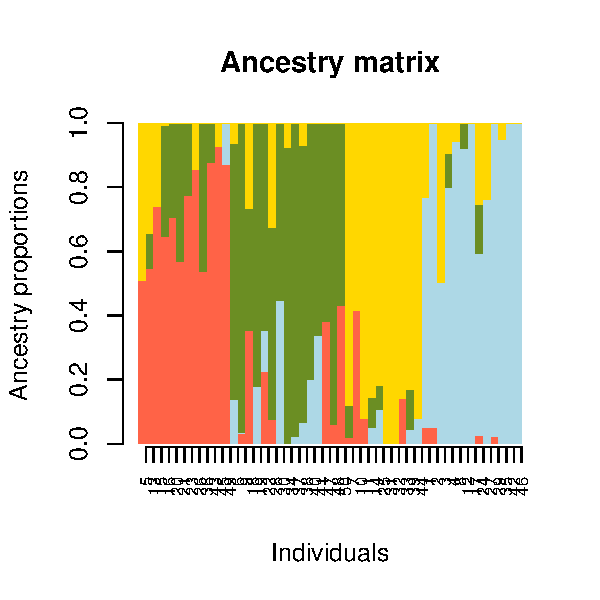
\includegraphics[width=\maxwidth]{figure/unnamed-chunk-10-1} 

\end{knitrout}
\caption{Ancestry coefficients obtained from {\tt snmf}.}
\end{figure}

Note that the conversion as a {\tt Qmatrix} object is also useful for running improved graphical functions from other packages such as {\tt tess3r} \citep{Caye_2016}.

\subsection{Population differentation tests using {\tt snmf}}

Approaches to sorting selective loci from the genomic background commonly focus on extreme values of the fixation index, $F_{\rm st}$, across loci. The {\tt snmf} function can compute fixation indices when the population is genetically continuous, when predefining subpopulations is a difficult task, and in the presence of admixed individuals in the sample (\citep{Martins_2016}). In this approach, population differentiation statistics are computed from ancestry coefficients obtained a {\tt snmf} project, and $p$-values are returned for all loci. Here is an example of outlier analysis with {\tt snmf}.

\begin{figure}[h!]
    \centering
\begin{knitrout}
\definecolor{shadecolor}{rgb}{0.969, 0.969, 0.969}\color{fgcolor}\begin{kframe}
\begin{alltt}
\hlcom{# Population differentiation tests}
\hlstd{p} \hlkwb{=} \hlkwd{snmf.pvalues}\hlstd{(project.snmf,}
                 \hlkwc{entropy} \hlstd{=} \hlnum{TRUE}\hlstd{,}
                 \hlkwc{ploidy} \hlstd{=} \hlnum{2}\hlstd{,}
                 \hlkwc{K} \hlstd{=} \hlnum{4}\hlstd{)}
\end{alltt}


{\ttfamily\noindent\bfseries\color{errorcolor}{\#\# Error in snmf.pvalues(project.snmf, entropy = TRUE, ploidy = 2, K = 4): erreur d'évaluation de l'argument 'object' lors de la sélection d'une méthode pour la fonction 'snmf.pvalues' : Erreur : objet 'project.snmf' introuvable}}\begin{alltt}
\hlkwd{par}\hlstd{(}\hlkwc{mfrow} \hlstd{=} \hlkwd{c}\hlstd{(}\hlnum{2}\hlstd{,}\hlnum{1}\hlstd{))}
\hlkwd{hist}\hlstd{(p}\hlopt{$}\hlstd{pvalues,} \hlkwc{col} \hlstd{=} \hlstr{"orange"}\hlstd{)}
\end{alltt}


{\ttfamily\noindent\bfseries\color{errorcolor}{\#\# Error in hist(p\$pvalues, col = "{}orange"{}): objet 'p' introuvable}}\begin{alltt}
\hlkwd{plot}\hlstd{(}\hlopt{-}\hlkwd{log10}\hlstd{(p}\hlopt{$}\hlstd{pvalues),} \hlkwc{pch} \hlstd{=} \hlnum{19}\hlstd{,} \hlkwc{col} \hlstd{=} \hlstr{"blue"}\hlstd{,} \hlkwc{cex} \hlstd{=} \hlnum{.7}\hlstd{)}
\end{alltt}


{\ttfamily\noindent\bfseries\color{errorcolor}{\#\# Error in plot(-log10(p\$pvalues), pch = 19, col = "{}blue"{}, cex = 0.7): erreur d'évaluation de l'argument 'x' lors de la sélection d'une méthode pour la fonction 'plot' : Erreur : objet 'p' introuvable}}\end{kframe}
\end{knitrout}
\caption{$P$-values for population differentiation tests.}
\end{figure}



\subsection{Missing genotype imputation using {\tt snmf}}

Missing genotypes are critical to genomewide association studies. Before running an association study, an important step is to replace the missing data, represented as "9" in the {\tt geno} and {\tt lfmm}) files, by better values. To provide an example of missing data imputation, let's start by removing 100 genotypes from the original data.
The resulting matrix is saved in the file "genotype_M.geno".
\begin{knitrout}
\definecolor{shadecolor}{rgb}{0.969, 0.969, 0.969}\color{fgcolor}\begin{kframe}
\begin{alltt}
\hlcom{# creation of a genotypic matrix  with missing genotypes}
\hlstd{dat} \hlkwb{=} \hlkwd{as.numeric}\hlstd{(tutorial.R)}
\hlstd{dat[}\hlkwd{sample}\hlstd{(}\hlnum{1}\hlopt{:}\hlkwd{length}\hlstd{(dat),} \hlnum{100}\hlstd{)]} \hlkwb{<-}  \hlnum{9}
\hlstd{dat} \hlkwb{<-} \hlkwd{matrix}\hlstd{(dat,} \hlkwc{nrow} \hlstd{=} \hlnum{50}\hlstd{,} \hlkwc{ncol} \hlstd{=} \hlnum{400}\hlstd{)}
\hlkwd{write.geno}\hlstd{(dat,} \hlstr{"genotype_M.geno"}\hlstd{)}
\end{alltt}
\begin{verbatim}
## [1] "genotype_M.geno"
\end{verbatim}
\end{kframe}
\end{knitrout}

Next, {\tt snmf} can be run on the data with missing genotypes as follows. The genotypic matrix completion is based on estimated ancestry coefficients and ancestral genotype frequencies.
\begin{knitrout}
\definecolor{shadecolor}{rgb}{0.969, 0.969, 0.969}\color{fgcolor}\begin{kframe}
\begin{alltt}
\hlstd{project.missing} \hlkwb{=} \hlkwd{snmf}\hlstd{(}\hlstr{"genotype_M.geno"}\hlstd{,} \hlkwc{K} \hlstd{=} \hlnum{4}\hlstd{,}
        \hlkwc{entropy} \hlstd{=} \hlnum{TRUE}\hlstd{,} \hlkwc{repetitions} \hlstd{=} \hlnum{10}\hlstd{,}
        \hlkwc{project} \hlstd{=} \hlstr{"new"}\hlstd{)}
\end{alltt}
\begin{verbatim}
## The project is saved into :
##  genotype_M.snmfProject 
## 
## To load the project, use:
##  project = load.snmfProject("genotype_M.snmfProject")
## 
## To remove the project, use:
##  remove.snmfProject("genotype_M.snmfProject")
## 
## [1] 2039721533
## [1] "*************************************"
## [1] "*          create.dataset            *"
## [1] "*************************************"
## summary of the options:
## 
##         -n (number of individuals)                 50
##         -L (number of loci)                        400
##         -s (seed random init)                      2039721533
##         -r (percentage of masked data)             0.05
##         -x (genotype file in .geno format)         /Users/francois/Datas/LEA/LEA/vignettes/genotype_M.geno
##         -o (output file in .geno format)           /Users/francois/Datas/LEA/LEA/vignettes/genotype_M.snmf/masked/genotype_M_I.geno
## 
##  Write genotype file with masked data, /Users/francois/Datas/LEA/LEA/vignettes/genotype_M.snmf/masked/genotype_M_I.geno:		OK.
## 
## [1] "*************************************"
## [1] "* sNMF K = 4  repetition 1      *"
## [1] "*************************************"
## summary of the options:
## 
##         -n (number of individuals)             50
##         -L (number of loci)                    400
##         -K (number of ancestral pops)          4
##         -x (input file)                        /Users/francois/Datas/LEA/LEA/vignettes/genotype_M.snmf/masked/genotype_M_I.geno
##         -q (individual admixture file)         /Users/francois/Datas/LEA/LEA/vignettes/genotype_M.snmf/K4/run1/genotype_M_r1.4.Q
##         -g (ancestral frequencies file)        /Users/francois/Datas/LEA/LEA/vignettes/genotype_M.snmf/K4/run1/genotype_M_r1.4.G
##         -i (number max of iterations)          200
##         -a (regularization parameter)          10
##         -s (seed random init)                  140232721935933
##         -e (tolerance error)                   1E-05
##         -p (number of processes)               1
##         - diploid
## 
## Read genotype file /Users/francois/Datas/LEA/LEA/vignettes/genotype_M.snmf/masked/genotype_M_I.geno:		OK.
## 
## 
## Main algorithm:
## 	[                                                                           ]
## 	[===================================]
## Number of iterations: 94
## 
## Least-square error: 5462.240537
## Write individual ancestry coefficient file /Users/francois/Datas/LEA/LEA/vignettes/genotype_M.snmf/K4/run1/genotype_M_r1.4.Q:		OK.
## Write ancestral allele frequency coefficient file /Users/francois/Datas/LEA/LEA/vignettes/genotype_M.snmf/K4/run1/genotype_M_r1.4.G:	OK.
## 
## [1] "*************************************"
## [1] "*    cross-entropy estimation       *"
## [1] "*************************************"
## summary of the options:
## 
##         -n (number of individuals)         50
##         -L (number of loci)                400
##         -K (number of ancestral pops)      4
##         -x (genotype file)                 /Users/francois/Datas/LEA/LEA/vignettes/genotype_M.geno
##         -q (individual admixture)          /Users/francois/Datas/LEA/LEA/vignettes/genotype_M.snmf/K4/run1/genotype_M_r1.4.Q
##         -g (ancestral frequencies)         /Users/francois/Datas/LEA/LEA/vignettes/genotype_M.snmf/K4/run1/genotype_M_r1.4.G
##         -i (with masked genotypes)         /Users/francois/Datas/LEA/LEA/vignettes/genotype_M.snmf/masked/genotype_M_I.geno
##         - diploid
## 
## Cross-Entropy (all data):	 0.452887
## Cross-Entropy (masked data):	 0.589622
## The project is saved into :
##  genotype_M.snmfProject 
## 
## To load the project, use:
##  project = load.snmfProject("genotype_M.snmfProject")
## 
## To remove the project, use:
##  remove.snmfProject("genotype_M.snmfProject")
## 
## [1] 153938503
## [1] "*************************************"
## [1] "*          create.dataset            *"
## [1] "*************************************"
## summary of the options:
## 
##         -n (number of individuals)                 50
##         -L (number of loci)                        400
##         -s (seed random init)                      153938503
##         -r (percentage of masked data)             0.05
##         -x (genotype file in .geno format)         /Users/francois/Datas/LEA/LEA/vignettes/genotype_M.geno
##         -o (output file in .geno format)           /Users/francois/Datas/LEA/LEA/vignettes/genotype_M.snmf/masked/genotype_M_I.geno
## 
##  Write genotype file with masked data, /Users/francois/Datas/LEA/LEA/vignettes/genotype_M.snmf/masked/genotype_M_I.geno:		OK.
## 
## [1] "*************************************"
## [1] "* sNMF K = 4  repetition 2      *"
## [1] "*************************************"
## summary of the options:
## 
##         -n (number of individuals)             50
##         -L (number of loci)                    400
##         -K (number of ancestral pops)          4
##         -x (input file)                        /Users/francois/Datas/LEA/LEA/vignettes/genotype_M.snmf/masked/genotype_M_I.geno
##         -q (individual admixture file)         /Users/francois/Datas/LEA/LEA/vignettes/genotype_M.snmf/K4/run2/genotype_M_r2.4.Q
##         -g (ancestral frequencies file)        /Users/francois/Datas/LEA/LEA/vignettes/genotype_M.snmf/K4/run2/genotype_M_r2.4.G
##         -i (number max of iterations)          200
##         -a (regularization parameter)          10
##         -s (seed random init)                  140230836152903
##         -e (tolerance error)                   1E-05
##         -p (number of processes)               1
##         - diploid
## 
## Read genotype file /Users/francois/Datas/LEA/LEA/vignettes/genotype_M.snmf/masked/genotype_M_I.geno:		OK.
## 
## 
## Main algorithm:
## 	[                                                                           ]
## 	[=======================================]
## Number of iterations: 105
## 
## Least-square error: 5457.757372
## Write individual ancestry coefficient file /Users/francois/Datas/LEA/LEA/vignettes/genotype_M.snmf/K4/run2/genotype_M_r2.4.Q:		OK.
## Write ancestral allele frequency coefficient file /Users/francois/Datas/LEA/LEA/vignettes/genotype_M.snmf/K4/run2/genotype_M_r2.4.G:	OK.
## 
## [1] "*************************************"
## [1] "*    cross-entropy estimation       *"
## [1] "*************************************"
## summary of the options:
## 
##         -n (number of individuals)         50
##         -L (number of loci)                400
##         -K (number of ancestral pops)      4
##         -x (genotype file)                 /Users/francois/Datas/LEA/LEA/vignettes/genotype_M.geno
##         -q (individual admixture)          /Users/francois/Datas/LEA/LEA/vignettes/genotype_M.snmf/K4/run2/genotype_M_r2.4.Q
##         -g (ancestral frequencies)         /Users/francois/Datas/LEA/LEA/vignettes/genotype_M.snmf/K4/run2/genotype_M_r2.4.G
##         -i (with masked genotypes)         /Users/francois/Datas/LEA/LEA/vignettes/genotype_M.snmf/masked/genotype_M_I.geno
##         - diploid
## 
## Cross-Entropy (all data):	 0.452089
## Cross-Entropy (masked data):	 0.649582
## The project is saved into :
##  genotype_M.snmfProject 
## 
## To load the project, use:
##  project = load.snmfProject("genotype_M.snmfProject")
## 
## To remove the project, use:
##  remove.snmfProject("genotype_M.snmfProject")
## 
## [1] 1989255669
## [1] "*************************************"
## [1] "*          create.dataset            *"
## [1] "*************************************"
## summary of the options:
## 
##         -n (number of individuals)                 50
##         -L (number of loci)                        400
##         -s (seed random init)                      1989255669
##         -r (percentage of masked data)             0.05
##         -x (genotype file in .geno format)         /Users/francois/Datas/LEA/LEA/vignettes/genotype_M.geno
##         -o (output file in .geno format)           /Users/francois/Datas/LEA/LEA/vignettes/genotype_M.snmf/masked/genotype_M_I.geno
## 
##  Write genotype file with masked data, /Users/francois/Datas/LEA/LEA/vignettes/genotype_M.snmf/masked/genotype_M_I.geno:		OK.
## 
## [1] "*************************************"
## [1] "* sNMF K = 4  repetition 3      *"
## [1] "*************************************"
## summary of the options:
## 
##         -n (number of individuals)             50
##         -L (number of loci)                    400
##         -K (number of ancestral pops)          4
##         -x (input file)                        /Users/francois/Datas/LEA/LEA/vignettes/genotype_M.snmf/masked/genotype_M_I.geno
##         -q (individual admixture file)         /Users/francois/Datas/LEA/LEA/vignettes/genotype_M.snmf/K4/run3/genotype_M_r3.4.Q
##         -g (ancestral frequencies file)        /Users/francois/Datas/LEA/LEA/vignettes/genotype_M.snmf/K4/run3/genotype_M_r3.4.G
##         -i (number max of iterations)          200
##         -a (regularization parameter)          10
##         -s (seed random init)                  140232671470069
##         -e (tolerance error)                   1E-05
##         -p (number of processes)               1
##         - diploid
## 
## Read genotype file /Users/francois/Datas/LEA/LEA/vignettes/genotype_M.snmf/masked/genotype_M_I.geno:		OK.
## 
## 
## Main algorithm:
## 	[                                                                           ]
## 	[=================]
## Number of iterations: 45
## 
## Least-square error: 5490.553285
## Write individual ancestry coefficient file /Users/francois/Datas/LEA/LEA/vignettes/genotype_M.snmf/K4/run3/genotype_M_r3.4.Q:		OK.
## Write ancestral allele frequency coefficient file /Users/francois/Datas/LEA/LEA/vignettes/genotype_M.snmf/K4/run3/genotype_M_r3.4.G:	OK.
## 
## [1] "*************************************"
## [1] "*    cross-entropy estimation       *"
## [1] "*************************************"
## summary of the options:
## 
##         -n (number of individuals)         50
##         -L (number of loci)                400
##         -K (number of ancestral pops)      4
##         -x (genotype file)                 /Users/francois/Datas/LEA/LEA/vignettes/genotype_M.geno
##         -q (individual admixture)          /Users/francois/Datas/LEA/LEA/vignettes/genotype_M.snmf/K4/run3/genotype_M_r3.4.Q
##         -g (ancestral frequencies)         /Users/francois/Datas/LEA/LEA/vignettes/genotype_M.snmf/K4/run3/genotype_M_r3.4.G
##         -i (with masked genotypes)         /Users/francois/Datas/LEA/LEA/vignettes/genotype_M.snmf/masked/genotype_M_I.geno
##         - diploid
## 
## Cross-Entropy (all data):	 0.453591
## Cross-Entropy (masked data):	 0.566615
## The project is saved into :
##  genotype_M.snmfProject 
## 
## To load the project, use:
##  project = load.snmfProject("genotype_M.snmfProject")
## 
## To remove the project, use:
##  remove.snmfProject("genotype_M.snmfProject")
## 
## [1] 1198786353
## [1] "*************************************"
## [1] "*          create.dataset            *"
## [1] "*************************************"
## summary of the options:
## 
##         -n (number of individuals)                 50
##         -L (number of loci)                        400
##         -s (seed random init)                      1198786353
##         -r (percentage of masked data)             0.05
##         -x (genotype file in .geno format)         /Users/francois/Datas/LEA/LEA/vignettes/genotype_M.geno
##         -o (output file in .geno format)           /Users/francois/Datas/LEA/LEA/vignettes/genotype_M.snmf/masked/genotype_M_I.geno
## 
##  Write genotype file with masked data, /Users/francois/Datas/LEA/LEA/vignettes/genotype_M.snmf/masked/genotype_M_I.geno:		OK.
## 
## [1] "*************************************"
## [1] "* sNMF K = 4  repetition 4      *"
## [1] "*************************************"
## summary of the options:
## 
##         -n (number of individuals)             50
##         -L (number of loci)                    400
##         -K (number of ancestral pops)          4
##         -x (input file)                        /Users/francois/Datas/LEA/LEA/vignettes/genotype_M.snmf/masked/genotype_M_I.geno
##         -q (individual admixture file)         /Users/francois/Datas/LEA/LEA/vignettes/genotype_M.snmf/K4/run4/genotype_M_r4.4.Q
##         -g (ancestral frequencies file)        /Users/francois/Datas/LEA/LEA/vignettes/genotype_M.snmf/K4/run4/genotype_M_r4.4.G
##         -i (number max of iterations)          200
##         -a (regularization parameter)          10
##         -s (seed random init)                  140231881000753
##         -e (tolerance error)                   1E-05
##         -p (number of processes)               1
##         - diploid
## 
## Read genotype file /Users/francois/Datas/LEA/LEA/vignettes/genotype_M.snmf/masked/genotype_M_I.geno:		OK.
## 
## 
## Main algorithm:
## 	[                                                                           ]
## 	[============================]
## Number of iterations: 75
## 
## Least-square error: 5459.522577
## Write individual ancestry coefficient file /Users/francois/Datas/LEA/LEA/vignettes/genotype_M.snmf/K4/run4/genotype_M_r4.4.Q:		OK.
## Write ancestral allele frequency coefficient file /Users/francois/Datas/LEA/LEA/vignettes/genotype_M.snmf/K4/run4/genotype_M_r4.4.G:	OK.
## 
## [1] "*************************************"
## [1] "*    cross-entropy estimation       *"
## [1] "*************************************"
## summary of the options:
## 
##         -n (number of individuals)         50
##         -L (number of loci)                400
##         -K (number of ancestral pops)      4
##         -x (genotype file)                 /Users/francois/Datas/LEA/LEA/vignettes/genotype_M.geno
##         -q (individual admixture)          /Users/francois/Datas/LEA/LEA/vignettes/genotype_M.snmf/K4/run4/genotype_M_r4.4.Q
##         -g (ancestral frequencies)         /Users/francois/Datas/LEA/LEA/vignettes/genotype_M.snmf/K4/run4/genotype_M_r4.4.G
##         -i (with masked genotypes)         /Users/francois/Datas/LEA/LEA/vignettes/genotype_M.snmf/masked/genotype_M_I.geno
##         - diploid
## 
## Cross-Entropy (all data):	 0.452834
## Cross-Entropy (masked data):	 0.609625
## The project is saved into :
##  genotype_M.snmfProject 
## 
## To load the project, use:
##  project = load.snmfProject("genotype_M.snmfProject")
## 
## To remove the project, use:
##  remove.snmfProject("genotype_M.snmfProject")
## 
## [1] 613620133
## [1] "*************************************"
## [1] "*          create.dataset            *"
## [1] "*************************************"
## summary of the options:
## 
##         -n (number of individuals)                 50
##         -L (number of loci)                        400
##         -s (seed random init)                      613620133
##         -r (percentage of masked data)             0.05
##         -x (genotype file in .geno format)         /Users/francois/Datas/LEA/LEA/vignettes/genotype_M.geno
##         -o (output file in .geno format)           /Users/francois/Datas/LEA/LEA/vignettes/genotype_M.snmf/masked/genotype_M_I.geno
## 
##  Write genotype file with masked data, /Users/francois/Datas/LEA/LEA/vignettes/genotype_M.snmf/masked/genotype_M_I.geno:		OK.
## 
## [1] "*************************************"
## [1] "* sNMF K = 4  repetition 5      *"
## [1] "*************************************"
## summary of the options:
## 
##         -n (number of individuals)             50
##         -L (number of loci)                    400
##         -K (number of ancestral pops)          4
##         -x (input file)                        /Users/francois/Datas/LEA/LEA/vignettes/genotype_M.snmf/masked/genotype_M_I.geno
##         -q (individual admixture file)         /Users/francois/Datas/LEA/LEA/vignettes/genotype_M.snmf/K4/run5/genotype_M_r5.4.Q
##         -g (ancestral frequencies file)        /Users/francois/Datas/LEA/LEA/vignettes/genotype_M.snmf/K4/run5/genotype_M_r5.4.G
##         -i (number max of iterations)          200
##         -a (regularization parameter)          10
##         -s (seed random init)                  140231295834533
##         -e (tolerance error)                   1E-05
##         -p (number of processes)               1
##         - diploid
## 
## Read genotype file /Users/francois/Datas/LEA/LEA/vignettes/genotype_M.snmf/masked/genotype_M_I.geno:		OK.
## 
## 
## Main algorithm:
## 	[                                                                           ]
## 	[======================================]
## Number of iterations: 102
## 
## Least-square error: 5479.788866
## Write individual ancestry coefficient file /Users/francois/Datas/LEA/LEA/vignettes/genotype_M.snmf/K4/run5/genotype_M_r5.4.Q:		OK.
## Write ancestral allele frequency coefficient file /Users/francois/Datas/LEA/LEA/vignettes/genotype_M.snmf/K4/run5/genotype_M_r5.4.G:	OK.
## 
## [1] "*************************************"
## [1] "*    cross-entropy estimation       *"
## [1] "*************************************"
## summary of the options:
## 
##         -n (number of individuals)         50
##         -L (number of loci)                400
##         -K (number of ancestral pops)      4
##         -x (genotype file)                 /Users/francois/Datas/LEA/LEA/vignettes/genotype_M.geno
##         -q (individual admixture)          /Users/francois/Datas/LEA/LEA/vignettes/genotype_M.snmf/K4/run5/genotype_M_r5.4.Q
##         -g (ancestral frequencies)         /Users/francois/Datas/LEA/LEA/vignettes/genotype_M.snmf/K4/run5/genotype_M_r5.4.G
##         -i (with masked genotypes)         /Users/francois/Datas/LEA/LEA/vignettes/genotype_M.snmf/masked/genotype_M_I.geno
##         - diploid
## 
## Cross-Entropy (all data):	 0.452038
## Cross-Entropy (masked data):	 0.611227
## The project is saved into :
##  genotype_M.snmfProject 
## 
## To load the project, use:
##  project = load.snmfProject("genotype_M.snmfProject")
## 
## To remove the project, use:
##  remove.snmfProject("genotype_M.snmfProject")
## 
## [1] 1963248173
## [1] "*************************************"
## [1] "*          create.dataset            *"
## [1] "*************************************"
## summary of the options:
## 
##         -n (number of individuals)                 50
##         -L (number of loci)                        400
##         -s (seed random init)                      1963248173
##         -r (percentage of masked data)             0.05
##         -x (genotype file in .geno format)         /Users/francois/Datas/LEA/LEA/vignettes/genotype_M.geno
##         -o (output file in .geno format)           /Users/francois/Datas/LEA/LEA/vignettes/genotype_M.snmf/masked/genotype_M_I.geno
## 
##  Write genotype file with masked data, /Users/francois/Datas/LEA/LEA/vignettes/genotype_M.snmf/masked/genotype_M_I.geno:		OK.
## 
## [1] "*************************************"
## [1] "* sNMF K = 4  repetition 6      *"
## [1] "*************************************"
## summary of the options:
## 
##         -n (number of individuals)             50
##         -L (number of loci)                    400
##         -K (number of ancestral pops)          4
##         -x (input file)                        /Users/francois/Datas/LEA/LEA/vignettes/genotype_M.snmf/masked/genotype_M_I.geno
##         -q (individual admixture file)         /Users/francois/Datas/LEA/LEA/vignettes/genotype_M.snmf/K4/run6/genotype_M_r6.4.Q
##         -g (ancestral frequencies file)        /Users/francois/Datas/LEA/LEA/vignettes/genotype_M.snmf/K4/run6/genotype_M_r6.4.G
##         -i (number max of iterations)          200
##         -a (regularization parameter)          10
##         -s (seed random init)                  32028019245
##         -e (tolerance error)                   1E-05
##         -p (number of processes)               1
##         - diploid
## 
## Read genotype file /Users/francois/Datas/LEA/LEA/vignettes/genotype_M.snmf/masked/genotype_M_I.geno:		OK.
## 
## 
## Main algorithm:
## 	[                                                                           ]
## 	[=================================]
## Number of iterations: 88
## 
## Least-square error: 5437.161704
## Write individual ancestry coefficient file /Users/francois/Datas/LEA/LEA/vignettes/genotype_M.snmf/K4/run6/genotype_M_r6.4.Q:		OK.
## Write ancestral allele frequency coefficient file /Users/francois/Datas/LEA/LEA/vignettes/genotype_M.snmf/K4/run6/genotype_M_r6.4.G:	OK.
## 
## [1] "*************************************"
## [1] "*    cross-entropy estimation       *"
## [1] "*************************************"
## summary of the options:
## 
##         -n (number of individuals)         50
##         -L (number of loci)                400
##         -K (number of ancestral pops)      4
##         -x (genotype file)                 /Users/francois/Datas/LEA/LEA/vignettes/genotype_M.geno
##         -q (individual admixture)          /Users/francois/Datas/LEA/LEA/vignettes/genotype_M.snmf/K4/run6/genotype_M_r6.4.Q
##         -g (ancestral frequencies)         /Users/francois/Datas/LEA/LEA/vignettes/genotype_M.snmf/K4/run6/genotype_M_r6.4.G
##         -i (with masked genotypes)         /Users/francois/Datas/LEA/LEA/vignettes/genotype_M.snmf/masked/genotype_M_I.geno
##         - diploid
## 
## Cross-Entropy (all data):	 0.450893
## Cross-Entropy (masked data):	 0.609333
## The project is saved into :
##  genotype_M.snmfProject 
## 
## To load the project, use:
##  project = load.snmfProject("genotype_M.snmfProject")
## 
## To remove the project, use:
##  remove.snmfProject("genotype_M.snmfProject")
## 
## [1] 1349374288
## [1] "*************************************"
## [1] "*          create.dataset            *"
## [1] "*************************************"
## summary of the options:
## 
##         -n (number of individuals)                 50
##         -L (number of loci)                        400
##         -s (seed random init)                      1349374288
##         -r (percentage of masked data)             0.05
##         -x (genotype file in .geno format)         /Users/francois/Datas/LEA/LEA/vignettes/genotype_M.geno
##         -o (output file in .geno format)           /Users/francois/Datas/LEA/LEA/vignettes/genotype_M.snmf/masked/genotype_M_I.geno
## 
##  Write genotype file with masked data, /Users/francois/Datas/LEA/LEA/vignettes/genotype_M.snmf/masked/genotype_M_I.geno:		OK.
## 
## [1] "*************************************"
## [1] "* sNMF K = 4  repetition 7      *"
## [1] "*************************************"
## summary of the options:
## 
##         -n (number of individuals)             50
##         -L (number of loci)                    400
##         -K (number of ancestral pops)          4
##         -x (input file)                        /Users/francois/Datas/LEA/LEA/vignettes/genotype_M.snmf/masked/genotype_M_I.geno
##         -q (individual admixture file)         /Users/francois/Datas/LEA/LEA/vignettes/genotype_M.snmf/K4/run7/genotype_M_r7.4.Q
##         -g (ancestral frequencies file)        /Users/francois/Datas/LEA/LEA/vignettes/genotype_M.snmf/K4/run7/genotype_M_r7.4.G
##         -i (number max of iterations)          200
##         -a (regularization parameter)          10
##         -s (seed random init)                  5644341584
##         -e (tolerance error)                   1E-05
##         -p (number of processes)               1
##         - diploid
## 
## Read genotype file /Users/francois/Datas/LEA/LEA/vignettes/genotype_M.snmf/masked/genotype_M_I.geno:		OK.
## 
## 
## Main algorithm:
## 	[                                                                           ]
## 	[=====================]
## Number of iterations: 56
## 
## Least-square error: 5473.122543
## Write individual ancestry coefficient file /Users/francois/Datas/LEA/LEA/vignettes/genotype_M.snmf/K4/run7/genotype_M_r7.4.Q:		OK.
## Write ancestral allele frequency coefficient file /Users/francois/Datas/LEA/LEA/vignettes/genotype_M.snmf/K4/run7/genotype_M_r7.4.G:	OK.
## 
## [1] "*************************************"
## [1] "*    cross-entropy estimation       *"
## [1] "*************************************"
## summary of the options:
## 
##         -n (number of individuals)         50
##         -L (number of loci)                400
##         -K (number of ancestral pops)      4
##         -x (genotype file)                 /Users/francois/Datas/LEA/LEA/vignettes/genotype_M.geno
##         -q (individual admixture)          /Users/francois/Datas/LEA/LEA/vignettes/genotype_M.snmf/K4/run7/genotype_M_r7.4.Q
##         -g (ancestral frequencies)         /Users/francois/Datas/LEA/LEA/vignettes/genotype_M.snmf/K4/run7/genotype_M_r7.4.G
##         -i (with masked genotypes)         /Users/francois/Datas/LEA/LEA/vignettes/genotype_M.snmf/masked/genotype_M_I.geno
##         - diploid
## 
## Cross-Entropy (all data):	 0.453905
## Cross-Entropy (masked data):	 0.566196
## The project is saved into :
##  genotype_M.snmfProject 
## 
## To load the project, use:
##  project = load.snmfProject("genotype_M.snmfProject")
## 
## To remove the project, use:
##  remove.snmfProject("genotype_M.snmfProject")
## 
## [1] 1441649775
## [1] "*************************************"
## [1] "*          create.dataset            *"
## [1] "*************************************"
## summary of the options:
## 
##         -n (number of individuals)                 50
##         -L (number of loci)                        400
##         -s (seed random init)                      1441649775
##         -r (percentage of masked data)             0.05
##         -x (genotype file in .geno format)         /Users/francois/Datas/LEA/LEA/vignettes/genotype_M.geno
##         -o (output file in .geno format)           /Users/francois/Datas/LEA/LEA/vignettes/genotype_M.snmf/masked/genotype_M_I.geno
## 
##  Write genotype file with masked data, /Users/francois/Datas/LEA/LEA/vignettes/genotype_M.snmf/masked/genotype_M_I.geno:		OK.
## 
## [1] "*************************************"
## [1] "* sNMF K = 4  repetition 8      *"
## [1] "*************************************"
## summary of the options:
## 
##         -n (number of individuals)             50
##         -L (number of loci)                    400
##         -K (number of ancestral pops)          4
##         -x (input file)                        /Users/francois/Datas/LEA/LEA/vignettes/genotype_M.snmf/masked/genotype_M_I.geno
##         -q (individual admixture file)         /Users/francois/Datas/LEA/LEA/vignettes/genotype_M.snmf/K4/run8/genotype_M_r8.4.Q
##         -g (ancestral frequencies file)        /Users/francois/Datas/LEA/LEA/vignettes/genotype_M.snmf/K4/run8/genotype_M_r8.4.G
##         -i (number max of iterations)          200
##         -a (regularization parameter)          10
##         -s (seed random init)                  140232123864175
##         -e (tolerance error)                   1E-05
##         -p (number of processes)               1
##         - diploid
## 
## Read genotype file /Users/francois/Datas/LEA/LEA/vignettes/genotype_M.snmf/masked/genotype_M_I.geno:		OK.
## 
## 
## Main algorithm:
## 	[                                                                           ]
## 	[====================================]
## Number of iterations: 97
## 
## Least-square error: 5497.542049
## Write individual ancestry coefficient file /Users/francois/Datas/LEA/LEA/vignettes/genotype_M.snmf/K4/run8/genotype_M_r8.4.Q:		OK.
## Write ancestral allele frequency coefficient file /Users/francois/Datas/LEA/LEA/vignettes/genotype_M.snmf/K4/run8/genotype_M_r8.4.G:	OK.
## 
## [1] "*************************************"
## [1] "*    cross-entropy estimation       *"
## [1] "*************************************"
## summary of the options:
## 
##         -n (number of individuals)         50
##         -L (number of loci)                400
##         -K (number of ancestral pops)      4
##         -x (genotype file)                 /Users/francois/Datas/LEA/LEA/vignettes/genotype_M.geno
##         -q (individual admixture)          /Users/francois/Datas/LEA/LEA/vignettes/genotype_M.snmf/K4/run8/genotype_M_r8.4.Q
##         -g (ancestral frequencies)         /Users/francois/Datas/LEA/LEA/vignettes/genotype_M.snmf/K4/run8/genotype_M_r8.4.G
##         -i (with masked genotypes)         /Users/francois/Datas/LEA/LEA/vignettes/genotype_M.snmf/masked/genotype_M_I.geno
##         - diploid
## 
## Cross-Entropy (all data):	 0.452322
## Cross-Entropy (masked data):	 0.582242
## The project is saved into :
##  genotype_M.snmfProject 
## 
## To load the project, use:
##  project = load.snmfProject("genotype_M.snmfProject")
## 
## To remove the project, use:
##  remove.snmfProject("genotype_M.snmfProject")
## 
## [1] 139184544
## [1] "*************************************"
## [1] "*          create.dataset            *"
## [1] "*************************************"
## summary of the options:
## 
##         -n (number of individuals)                 50
##         -L (number of loci)                        400
##         -s (seed random init)                      139184544
##         -r (percentage of masked data)             0.05
##         -x (genotype file in .geno format)         /Users/francois/Datas/LEA/LEA/vignettes/genotype_M.geno
##         -o (output file in .geno format)           /Users/francois/Datas/LEA/LEA/vignettes/genotype_M.snmf/masked/genotype_M_I.geno
## 
##  Write genotype file with masked data, /Users/francois/Datas/LEA/LEA/vignettes/genotype_M.snmf/masked/genotype_M_I.geno:		OK.
## 
## [1] "*************************************"
## [1] "* sNMF K = 4  repetition 9      *"
## [1] "*************************************"
## summary of the options:
## 
##         -n (number of individuals)             50
##         -L (number of loci)                    400
##         -K (number of ancestral pops)          4
##         -x (input file)                        /Users/francois/Datas/LEA/LEA/vignettes/genotype_M.snmf/masked/genotype_M_I.geno
##         -q (individual admixture file)         /Users/francois/Datas/LEA/LEA/vignettes/genotype_M.snmf/K4/run9/genotype_M_r9.4.Q
##         -g (ancestral frequencies file)        /Users/francois/Datas/LEA/LEA/vignettes/genotype_M.snmf/K4/run9/genotype_M_r9.4.G
##         -i (number max of iterations)          200
##         -a (regularization parameter)          10
##         -s (seed random init)                  4607182418939201952
##         -e (tolerance error)                   1E-05
##         -p (number of processes)               1
##         - diploid
## 
## Read genotype file /Users/francois/Datas/LEA/LEA/vignettes/genotype_M.snmf/masked/genotype_M_I.geno:		OK.
## 
## 
## Main algorithm:
## 	[                                                                           ]
## 	[===============================================]
## Number of iterations: 126
## 
## Least-square error: 5455.188627
## Write individual ancestry coefficient file /Users/francois/Datas/LEA/LEA/vignettes/genotype_M.snmf/K4/run9/genotype_M_r9.4.Q:		OK.
## Write ancestral allele frequency coefficient file /Users/francois/Datas/LEA/LEA/vignettes/genotype_M.snmf/K4/run9/genotype_M_r9.4.G:	OK.
## 
## [1] "*************************************"
## [1] "*    cross-entropy estimation       *"
## [1] "*************************************"
## summary of the options:
## 
##         -n (number of individuals)         50
##         -L (number of loci)                400
##         -K (number of ancestral pops)      4
##         -x (genotype file)                 /Users/francois/Datas/LEA/LEA/vignettes/genotype_M.geno
##         -q (individual admixture)          /Users/francois/Datas/LEA/LEA/vignettes/genotype_M.snmf/K4/run9/genotype_M_r9.4.Q
##         -g (ancestral frequencies)         /Users/francois/Datas/LEA/LEA/vignettes/genotype_M.snmf/K4/run9/genotype_M_r9.4.G
##         -i (with masked genotypes)         /Users/francois/Datas/LEA/LEA/vignettes/genotype_M.snmf/masked/genotype_M_I.geno
##         - diploid
## 
## Cross-Entropy (all data):	 0.452659
## Cross-Entropy (masked data):	 0.616562
## The project is saved into :
##  genotype_M.snmfProject 
## 
## To load the project, use:
##  project = load.snmfProject("genotype_M.snmfProject")
## 
## To remove the project, use:
##  remove.snmfProject("genotype_M.snmfProject")
## 
## [1] 1198276514
## [1] "*************************************"
## [1] "*          create.dataset            *"
## [1] "*************************************"
## summary of the options:
## 
##         -n (number of individuals)                 50
##         -L (number of loci)                        400
##         -s (seed random init)                      1198276514
##         -r (percentage of masked data)             0.05
##         -x (genotype file in .geno format)         /Users/francois/Datas/LEA/LEA/vignettes/genotype_M.geno
##         -o (output file in .geno format)           /Users/francois/Datas/LEA/LEA/vignettes/genotype_M.snmf/masked/genotype_M_I.geno
## 
##  Write genotype file with masked data, /Users/francois/Datas/LEA/LEA/vignettes/genotype_M.snmf/masked/genotype_M_I.geno:		OK.
## 
## [1] "*************************************"
## [1] "* sNMF K = 4  repetition 10      *"
## [1] "*************************************"
## summary of the options:
## 
##         -n (number of individuals)             50
##         -L (number of loci)                    400
##         -K (number of ancestral pops)          4
##         -x (input file)                        /Users/francois/Datas/LEA/LEA/vignettes/genotype_M.snmf/masked/genotype_M_I.geno
##         -q (individual admixture file)         /Users/francois/Datas/LEA/LEA/vignettes/genotype_M.snmf/K4/run10/genotype_M_r10.4.Q
##         -g (ancestral frequencies file)        /Users/francois/Datas/LEA/LEA/vignettes/genotype_M.snmf/K4/run10/genotype_M_r10.4.G
##         -i (number max of iterations)          200
##         -a (regularization parameter)          10
##         -s (seed random init)                  140231880490914
##         -e (tolerance error)                   1E-05
##         -p (number of processes)               1
##         - diploid
## 
## Read genotype file /Users/francois/Datas/LEA/LEA/vignettes/genotype_M.snmf/masked/genotype_M_I.geno:		OK.
## 
## 
## Main algorithm:
## 	[                                                                           ]
## 	[======================]
## Number of iterations: 59
## 
## Least-square error: 5493.012769
## Write individual ancestry coefficient file /Users/francois/Datas/LEA/LEA/vignettes/genotype_M.snmf/K4/run10/genotype_M_r10.4.Q:		OK.
## Write ancestral allele frequency coefficient file /Users/francois/Datas/LEA/LEA/vignettes/genotype_M.snmf/K4/run10/genotype_M_r10.4.G:	OK.
## 
## [1] "*************************************"
## [1] "*    cross-entropy estimation       *"
## [1] "*************************************"
## summary of the options:
## 
##         -n (number of individuals)         50
##         -L (number of loci)                400
##         -K (number of ancestral pops)      4
##         -x (genotype file)                 /Users/francois/Datas/LEA/LEA/vignettes/genotype_M.geno
##         -q (individual admixture)          /Users/francois/Datas/LEA/LEA/vignettes/genotype_M.snmf/K4/run10/genotype_M_r10.4.Q
##         -g (ancestral frequencies)         /Users/francois/Datas/LEA/LEA/vignettes/genotype_M.snmf/K4/run10/genotype_M_r10.4.G
##         -i (with masked genotypes)         /Users/francois/Datas/LEA/LEA/vignettes/genotype_M.snmf/masked/genotype_M_I.geno
##         - diploid
## 
## Cross-Entropy (all data):	 0.453098
## Cross-Entropy (masked data):	 0.581895
## The project is saved into :
##  genotype_M.snmfProject 
## 
## To load the project, use:
##  project = load.snmfProject("genotype_M.snmfProject")
## 
## To remove the project, use:
##  remove.snmfProject("genotype_M.snmfProject")
\end{verbatim}
\end{kframe}
\end{knitrout}
Then the project data can be used to impute the missing data as follows. 

\begin{knitrout}
\definecolor{shadecolor}{rgb}{0.969, 0.969, 0.969}\color{fgcolor}\begin{kframe}
\begin{alltt}
\hlcom{# select the run with the lowest cross-entropy value}
\hlstd{best} \hlkwb{=} \hlkwd{which.min}\hlstd{(}\hlkwd{cross.entropy}\hlstd{(project.missing,} \hlkwc{K} \hlstd{=} \hlnum{4}\hlstd{))}

\hlcom{# Impute the missing genotypes}
\hlkwd{impute}\hlstd{(project,} \hlstr{"genotype_M.lfmm"}\hlstd{,} \hlkwc{method} \hlstd{=} \hlstr{'mode'}\hlstd{,} \hlkwc{K} \hlstd{=} \hlnum{4}\hlstd{,} \hlkwc{run} \hlstd{= best)}
\end{alltt}


{\ttfamily\noindent\bfseries\color{errorcolor}{\#\# Error in impute(project, "{}genotype\_M.lfmm"{}, method = "{}mode"{}, K = 4, run = best): Input file not found.}}\begin{alltt}
\hlcom{# Compare with truth: proportion of correct imputation results}
\hlstd{dat.imp} \hlkwb{=} \hlkwd{read.lfmm}\hlstd{(}\hlstr{"genotypes_M.lfmm_imputed.lfmm"}\hlstd{)}
\end{alltt}


{\ttfamily\noindent\color{warningcolor}{\#\# Warning in file(file, "{}rt"{}): impossible d'ouvrir le fichier 'genotypes\_M.lfmm\_imputed.lfmm' : No such file or directory}}

{\ttfamily\noindent\bfseries\color{errorcolor}{\#\# Error in file(file, "{}rt"{}): impossible d'ouvrir la connexion}}\begin{alltt}
\hlkwd{mean}\hlstd{( tutorial.R[dat} \hlopt{==} \hlnum{9}\hlstd{]} \hlopt{==} \hlstd{dat.imp[dat} \hlopt{==} \hlnum{9}\hlstd{] )}
\end{alltt}


{\ttfamily\noindent\bfseries\color{errorcolor}{\#\# Error in mean(tutorial.R[dat == 9] == dat.imp[dat == 9]): objet 'dat.imp' introuvable}}\end{kframe}
\end{knitrout}
 
The results are saved in an output file with the string "_imputed" in its suffix name.

\section{Ecological associations tests using lfmm}

The {\tt R} package {\tt LEA} performs genomewide association analysis based on latent factor mixed models using the {\tt lfmm} function \citep{Frichot_2013}. To recall the model, let $G$ denote the genotypic matrix, storing allele frequencies for each individual at each locus, and let $X$ denote a set of $d$ ecological predictors or phenotypic traits. LFMMs consider the genotypic matrix entries as response variables in a linear regression model
\begin{equation}
 G_{i\ell} = \mu_\ell + \beta_{\ell}^TX_{i} + U_i^TV_\ell + \epsilon_{i\ell} \, ,
 \end{equation}
where $\mu_\ell$ is a locus specific effect, $\beta_\ell$ is a $d$-dimensional vector of regression coefficients, $U_i$ contains $K$ latent factors, and $V_\ell$ contains their corresponding loadings ($i$ stands for an individual and $\ell$ for a locus). The residual terms, $\epsilon_{i\ell}$, are statistically independent Gaussian variables with mean zero and variance $\sigma^2$.
\newline
\newline
 In latent factor models, association between predictors and allele frequencies can be tested while estimating unobserved latent factors that model confounding effects. In principle, the latent factors include levels of population structure due to shared demographic history or background genetic variation. After correction for confounding effects, association between allele frequencies and an ecological predictorat a particular locus is often interpreted as a signature of natural selection.


\paragraph{The run.}  The {\tt lfmm} program is based on a stochastic algorithm (MCMC) which doesnot provide exact results. We recommend using large number of cycles (e.g., {\tt -i 6000}) and the burnin period should set at least to one-half of the total number of cycles ({\tt -b 3000}). We have noticed that the program results are sensitive to the run-length parameter when data sets have relatively small sizes (eg, a few hundreds of individuals, a few thousands of loci). We recommend increasing  the burn-in period and the total number of cycles in this situation.


\begin{knitrout}
\definecolor{shadecolor}{rgb}{0.969, 0.969, 0.969}\color{fgcolor}\begin{kframe}
\begin{alltt}
\hlcom{# main options: }
\hlcom{# K: (the number of latent factors)}
\hlcom{# Runs with K = 4 and 5 repetitions.}
\hlstd{project} \hlkwb{=} \hlkwa{NULL}
\hlstd{project} \hlkwb{=} \hlkwd{lfmm}\hlstd{(}\hlstr{"genotypes.lfmm"}\hlstd{,}
               \hlstr{"gradients.env"}\hlstd{,}
                \hlkwc{K} \hlstd{=} \hlnum{4}\hlstd{,}
                \hlkwc{repetitions} \hlstd{=} \hlnum{5}\hlstd{,}
                \hlkwc{project} \hlstd{=} \hlstr{"new"}\hlstd{)}
\end{alltt}
\end{kframe}
\end{knitrout}

\paragraph{Deciding the number of latent factors.} Deciding an appropriate value for the number of latent factors in the {\tt lfmm} call can be based on the analysis of histograms of test significance values. Ideally, histograms should be flat, with a peak close to zero.

Since the objective is to control the false discovery rate (FDR) while keeping reasonable power to reject the null hypothesis, we recommend using several runs for each value of $K$ and combine $p$-values (use 5 to 10 runs, see our script below).  Choosing values of $K$ for which the histograms show their correct shape warrants that the FDR can be controlled efficiently.\\


Testing all $K$ values in a large range, from 1 to 20 for example, is generally useless. A careful analysis of population structure and estimates of the number of ancestral populations contributing to the genetic data indicates the range of values to be explored. For example the {\tt snmf} program estimates 4 ancestral populations, then running {\tt lfmm} for $K = 3-5$ often provides good results.


\paragraph{Combining $z$-scores obtained from multiple runs.}  We use the Fisher-Stouffer or a similar method to combine $z$-scores from multiple runs. In practice, we found that using the median $z$-scores of 5-10 runs and re-adjusting the $p$-values afterwards increase the power of {\tt lfmm} tests. This procedure is implemented in {\tt LEA} function, {\tt lfmm.pvalues}.

The $p$-values were adjusted as follows
\begin{knitrout}
\definecolor{shadecolor}{rgb}{0.969, 0.969, 0.969}\color{fgcolor}\begin{kframe}
\begin{alltt}
\hlcom{# compute adjusted p-values}
\hlstd{p} \hlkwb{=} \hlkwd{lfmm.pvalues}\hlstd{(project,} \hlkwc{K} \hlstd{=} \hlnum{4}\hlstd{)}
\hlstd{pvalues} \hlkwb{=} \hlstd{p}\hlopt{$}\hlstd{pvalues}
\end{alltt}
\end{kframe}
\end{knitrout}
The results can be displayed as follows.
\begin{figure}[h!]
    \centering
\begin{knitrout}
\definecolor{shadecolor}{rgb}{0.969, 0.969, 0.969}\color{fgcolor}\begin{kframe}
\begin{alltt}
\hlcom{# GWAS significance test}
\hlkwd{par}\hlstd{(}\hlkwc{mfrow} \hlstd{=} \hlkwd{c}\hlstd{(}\hlnum{2}\hlstd{,}\hlnum{1}\hlstd{))}
\hlkwd{hist}\hlstd{(p}\hlopt{$}\hlstd{pvalues,} \hlkwc{col} \hlstd{=} \hlstr{"lightblue"}\hlstd{)}
\hlkwd{plot}\hlstd{(}\hlopt{-}\hlkwd{log10}\hlstd{(pvalues),} \hlkwc{pch} \hlstd{=} \hlnum{19}\hlstd{,} \hlkwc{col} \hlstd{=} \hlstr{"blue"}\hlstd{,} \hlkwc{cex} \hlstd{=} \hlnum{.7}\hlstd{)}
\end{alltt}
\end{kframe}
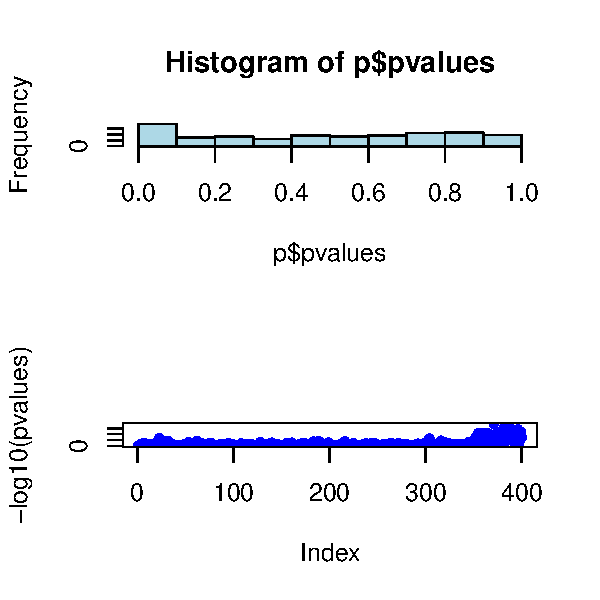
\includegraphics[width=\maxwidth]{figure/unnamed-chunk-17-1} 

\end{knitrout}
\caption{$P$-values for LFMM tests.}
\end{figure}

\noindent
To adjust $p$-values for multiple testing issues, we can use the Benjamini-Hochberg procedure. Here we set the expected levels of FDR equal to $q = 5 \%$, $10 \%$, $15 \%$ and $20 \%$ respectively \citep{Benjamini_1995}. The lists of candidate loci are given by the following script.
\begin{knitrout}
\definecolor{shadecolor}{rgb}{0.969, 0.969, 0.969}\color{fgcolor}\begin{kframe}
\begin{alltt}
\hlkwd{for} (alpha in \hlkwd{c}(.05,.1,.15,.2)) \{
\hlcom{    # expected FDR}
    \hlkwd{print}(\hlkwd{paste}(\hlstr{"expected FDR:"}, alpha))
    L = \hlkwd{length}(pvalues)
\hlcom{    # return a list of candidates with expected FDR alpha.}
\hlcom{    # Benjamini-Hochberg's algorithm:}
    w = \hlkwd{which}(\hlkwd{sort}(pvalues) < alpha * (1:L) / L)
    candidates = \hlkwd{order}(pvalues)[w]
\end{alltt}


{\ttfamily\noindent\bfseries\color{errorcolor}{\#\# Error: <text>:9:0: unexpected end of input\\\#\# 7:\ \ \ \  w = which(sort(pvalues) < alpha * (1:L) / L)\\\#\# 8:\ \ \ \  candidates = order(pvalues)[w]\\\#\#\ \  \textasciicircum{}}}\end{kframe}
\end{knitrout}

Since we have simulated data with their ground truth, we can compare the expected FDR levels to their observed levels, and compute the power (TPR) of the test.
\begin{knitrout}
\definecolor{shadecolor}{rgb}{0.969, 0.969, 0.969}\color{fgcolor}\begin{kframe}
\begin{alltt}
\hlcom{    # estimated FDR and True Positif}
    estimated.FDR = \hlkwd{length}(\hlkwd{which}(candidates <= 350))/\hlkwd{length}(candidates)
    estimated.TPR = \hlkwd{length}(\hlkwd{which}(candidates > 350))/50
    \hlkwd{print}(\hlkwd{paste}(\hlstr{"FDR:"}, estimated.FDR, \hlstr{"True Positive Rate:"}, estimated.TPR))
\}
\end{alltt}


{\ttfamily\noindent\bfseries\color{errorcolor}{\#\# Error: <text>:5:1: '\}' inattendu(e)\\\#\# 4:\ \ \ \  print(paste("{}FDR:"{}, estimated.FDR, "{}True Positive Rate:"{}, estimated.TPR))\\\#\# 5: \}\\\#\#\ \ \ \ \textasciicircum{}}}\end{kframe}
\end{knitrout}





\bibliographystyle{cse}
\bibliography{biblio}

\end{document}
